\chapter{Method}

This chapter will introduce and develop the \rrtfunnel\ algorithm, through two
means: Developing robust motion primitives through the \ac{SOS} programming
framework, based on the work in~\cite{majumdarFunnelLibrariesRealtime2017}, and
second deploy these funnels as motion primitives in a discrete \ac{RRT} planner,
based on~\cite{lavalleLav98cPdf}. This is beneficial, as using \textit{robust}
motion primitives has several advantages. Firstly, they are robust to
uncertainty, and thus, as long as the uncertainties in the system are akin to
our assumptions, the vehicle will not leave the funnel path. Secondly, with the
assumption that the primitives are robust, there is no need for more
conservative maneuvers and heuristics, such as maximizing the distance to an
obstacle. This means that a robust motion primitive algorithm can perform more
aggressive maneuvers than one that is inherently cautious about its
environment~\cite{majumdarFunnelLibrariesRealtime2017}.

\section{Defining funnels}

The funnel computations will be based on the \ac{SOS} theory as developed
in~\ref{sec:Funnels}. Given a trajectory, the goal is to compute a robust
invariant set around the trajectory that will `guarantee' that the planner is
free from collisions during execution of the obtained motion plan. This robustly
invariant set is parameterized through Lyapunov function candidates, that, in
this case, will be based upon the \ac{PSD} matrix that the time-invariant
\ac{LQR} controller produces. The following presentations will be based
on~\cite{tobenkinInvariantFunnelsTrajectories2010,
  tedrakeLQRtreesFeedbackMotion2009, majumdarRobustOnlineMotion2013}, but mainly
follow the formulations, and syntax
from~\cite{majumdarFunnelLibrariesRealtime2017}.

Thus, given the nonlinear dynamical system
\begin{equation}
  \label{eq:dynamicalsystem}
  \dot{x} = f(x(t), u(t))
\end{equation}
with \(x(t)\) the state of the system at time \(t\) and \(u(t)\) the control
input. Assume that a open loop nominal trajectory \(x_0 \colon [0,T] \rightarrow
\R^n\) with control input \(u_0 \colon [0,T] \rightarrow \R^n\) is given, and
define a change of coordinates into the error coordinate frame
\[
  \bar{x}(t) = (x - x_0)(t) \\
  \bar{u}(t) = (u - u_0)(t).
\]
Then, changing~\ref{eq:dynamicalsystem} to these new coordinates one obtaines
\begin{equation}
  \dot{\bar{x}} = \dot{x} - \dot{x}_0 = f(x_0(t) + \bar{x}(t), u_0(t) + \bar{u}(t)) - \dot{x}_0(t)
\end{equation}

In order to compute a parameterized reachable set through \ac{SOS} programming
the system~\ref{eq:dynamicalsystem} needs to be polynomial, and parameterized by
\(x\) and \(t\), since the trajectory is parametrized by \(x\) and \(t\).
Therefore, through the use of a \ac{TV-LQR} controller, the control input can be
eliminated from the dynamical equation, giving
\begin{equation}
  \label{eq:dynamicclosedloop}
  \dot{\bar{x}} = f_{cl}(t,\bar{x}(t)).
\end{equation}
However, the dynamical system may still not be polynomial, which is a necessary
condition in order for this to be verified using \ac{SOS} programming. Expanding
the system~\ref{eq:dynamicclosedloop} around the nominal trajectory \(x_0\)
through a Taylor expansion of some degree high enough to capture the
nonlinearities of the system.

The goal is to parametrize a tight outer approximation of the set of states the
system may transition into during the time interval \([0,T]\). Given that
\(F(t)\) is the set of states the system (\ref{eq:dynamicclosedloop}) can be in
at time \(t\), then
\begin{equation}
  \label{eq:reachableset}
  \bar{x}(0) \in \mathcal{X}_0 \implies \x(t) \in F(t), \, \forall t \in [0,T]
\end{equation}~\cite{majumdarFunnelLibrariesRealtime2017} 
where \(\mathcal{X}_0\) is the initial condition set, and \(F(t) \subset \R^n\).

A funnel is defined in~\cite{majumdarFunnelLibrariesRealtime2017} as
\begin{definition}
  \label{def:funnel}
  A funnel associatied with a closed-loop dynamical system \(\dot{\bar{x}} =
  f_{cl}(t,x(t))\) is a map \(F \colon [0,T] \rightarrow \mathcal{P}(\R^n)\),
  from the time interval \([0,T]\) to the power set (i.e., the set of subsets)
  of \(\R^n\) so that the sets \(F(t)\) satisfy the
  condition~\ref{eq:reachableset}.
\end{definition}
Thus, \(F(t)\) is the set of reachable states that the system can be in at time
\(t\).

Next, the reachable set is paramterized through the use of Lyapunov functions,
which yields
\begin{equation}
  F(t) = \set{\bar{x}(t) \mid V(t, \bar{x}(t) \leq \rho (t))}
\end{equation}
where \(\rho (t) \colon [0,T] \rightarrow \R^+\), is a function which limits the
size of the reachable set, and \(V(t,\bar{x}(t))\) is a Lyapunov function \(V
\colon [0,T] \times \R^n \rightarrow \R^+\).

Then, by setting \(\mathcal{X}_0 \subset F(0,\bar{x})\), one can derive the
sufficient condition for containing the reachable~\ref{eq:reachableset} set in
the Lyapunov function paramterization
\begin{equation}
  V(t,\bar{x}) = \rho(t) \implies \dot{V}(t,\bar{x}) < \dot{rho}(t), \, \forall t \in [0,T]
\end{equation}
with \(\dot{V}(t,\bar{x})\) computed as
\begin{equation}
  \label{eq:funnelsufficient}
  \dot{V}(t,\bar{x}) = \frac{\partial V(t,\bar{x})}{\partial x} f_{cl}(t,\bar{x}) + \frac{\partial V(t,\bar{x})}{\partial t}
\end{equation}

Currently there are no limitations on the functions \(V\) and \(\rho\), and
hence there exists infinitely many functions with different sized reachable sets
that satisfies~\ref{eq:funnelsifficient}, and is a valid funnel in the sense of
definition~\ref{def:funnel}. In order for efficient planning to take place, the
motion primitives, meaning the size of the funnels, should be as small as
possible, and it is therefore that the size of the funnels is minimized using
the following optimization problem~\cite{majumdarFunnelLibrariesRealtime2017}

\begin{align}
  \label{eq:funneloptimizationproblem}
  &\underset{V,\rho}{\text{inf}} \; &&\int_{0}^{T} vol(F(t)) dt \\
  &\text{subject to} && V(t,\bar{x}) = \rho (t) \implies \dot{V}(t,\bar{x}) < \rho (t), \, \forall t \in [0,T] \\
  && &\mathcal{X}_0 \subset F(0,\bar{x}) \\
\end{align} 


\section{Computing funnels}

\subsection{Formulating the optimization problem as a SOS program}

The optimization problem in~\ref{eq:funneloptimizationproblem} would prove
impossible to solve efficiently had it not been for advances in mathematical
convex numerical optimization, as in general the problem involves searching over
an infinite function space. While the general optimization problem of searching
through the infinite function space is not amenable to efficient numerical
computation, the problem can be made computationally feasible through the use of
a \ac{SOS} programming approach.

Thus in order to make the problem amenable to a \ac{SOS} program, there are some
assumptions that need to be met by our problem formulation. Firstly the initial
condition set needs to be a \textit{semi-algebraic set}, (\ie{} parameterized by
polynomial inequalities),

\begin{equation}
  \mathcal{X}_0 = \set{\bar{x} \in \R^n \mid g_{o,i}(\bar{x}) \geq 0, \, i = 1,\ldots,N_0}
\end{equation}

Then rewriting~(\ref{eq:funneloptimizationproblem})~as in terms of positivity
and equality constraints yields
\begin{equation}
  V(t,\bar{x}) = \rho(t) \implies \dot{\rho}(t) - \dot{V}(t,\bar{x}) > 0
\end{equation}
and
\begin{equation}
  g_{0,i}(\bar{x}) \geq 0 \forall i \in \set{1,\ldots,N_0} \implies \rho(0) - V(0,\bar{x}) \geq 0
\end{equation}
which, if these functions are both polynomial, is now in the form of a \ac{SOS}
optimization problem. Then through the use of the \textit{S-procedure} one
arrives at the equations
\begin{align}
  &\dot{\rho}(t) - \dot{V}(t,\bar{x}) - L(t,\bar{x})\left[ V(t,\bar{x}) - \rho(t) \right] - L_{t}(t,\bar{x})\left[ t\left( T - t \right) \right]  && \text{is SOS}& \label{eq:sufficient-conditions}\\
  & \rho(0) - V(0,\bar{x}) - \sum_{i}^{N_{0}} L_{0,i}(\bar{x})g_{0,i}(\bar{x}) && \text{is SOS}& \\
  & L_{t}(\bar{x}), \, L_{0,i}(\bar{x}) \; &&\text{are SOS}, \, \forall i \in \set{1,\ldots,N_{0}} \label{eq:sufficient-conditions3} \\
\end{align} 
where \(L\), \(L_{t}\), and \(L_{0,i}\) are multiplier
polynomials~(\ref{sec:s-procedure})~.

The goal is to make the parametrization of the reachable set as small as
possible, and therefore minimizing the cost
function~(\ref{eq:funneloptimizationproblem})~. This is done
in~\cite{majumdarFunnelLibrariesRealtime2017}, through approximating the cost
function by first discretizing the problem and replacing the integral with a
finite sum
\begin{equation}
  \label{eq:discrete-costfunction}
  \int_{0}^{T} vol(F(t)) dt \rightarrow \sum_{k=1}^{N} vol(F(t_{k}))
\end{equation}
Since the Lyapunov function \(V\) in this thesis will be quadratic, \(V\) can be
written as
\begin{equation}
  V(t_{k}, \bar{x}) = {\bar{x}}^{T}S_{k}\bar{x}, \, S_{k} \succeq 0
\end{equation}
which means that the set \(F(t_{k})\) is an ellipsoid in which the volume can be
minimized through maximizing the determinant of \(S_{k}\). Which in turn can be
transformed into a \ac{SDP} problem. If an upper bound on the cost
function~(\ref{eq:discrete-costfunction}) is introduced as
\begin{equation}
  \mathcal{E} (t_{k}) = \set{\bar{x} \in \R^n \mid {\bar{x}}^{T}S_{k}\bar{x} \leq 1, \, S_{k} \succeq 0}
\end{equation}
where \( \mathcal{E} ( t_{k} ) \) is an ellipsoid containing the reachable set
\( F ( t_{k} ) \) at time \( t_{k} \). This containment constraint can be
equivalently expressed as
\begin{equation}
  V ( t_{k}, \bar{x} ) \leq \rho(t_{k})  \implies {\bar{x}}^{T}S_{k}\bar{x} \leq 1.
\end{equation}
Which when expressed using \ac{SOS} constraints is
\begin{align}
  1 - {\bar{x}}^{T}S_{k}\bar{x} - L_{\mathcal{E},k}(\bar{x})\left[ \rho(t_{k}) - V(t_{k}, \bar{x}) \right]  \qquad \text{is SOS}& \\
  L_{\mathcal{E},k}(\bar{x}) \qquad \text{is SOS.}& \\
\end{align}

Then combining the cost function~(\ref{discrete-costfunction}) with the
constraints~(\ref{eq:sufficient-conditions}-\ref{eq:sufficient-conditions3}),
one arrives at

% TODO - maybe use optidef?
\begin{align}
  \underset{\substack{V,\rho,L,L_{t},\\L_{0,i},S_{k},L_{\mathcal{E},k}}}{\inf}&  \sum_{k=1}^{N} \mathrm{vol}(\mathcal{E}(t_{k}))& \\
  \sum_{k=1}^{N} vol(\set{ \bar{x} \mid {\bar{x}}^{T}S_{k}\bar{x} \leq 1})&& \\
  \text{such that}&\\
  \dot{\rho}(t) - \dot{V}(t,\bar{x}) - L(t,\bar{x}) \left[ V(t,\bar{x}) - \rho(t) \right] - L_{t}(t,\bar{x})\left[ t\left( T - t \right) \right] \qquad \text{is SOS}& \\
  \rho(0) - V(0,\bar{x}) - \sum_{i}^{N}L_{0,i}(\bar{x})g_{0,i}(\bar{x})& \text{is SOS}& \\
  1 - {\bar{x}}^{T}S_{k}\bar{x} - L_{\mathcal{E},k}(\bar{x}) \left[ \rho(t_{k}) - V(t_{k},\bar{x}) \right]& \text{is SOS}& \\
                                                                              &\forall k \in \set{1,\ldots,N} \, S_{k} \succeq 0& \\
  \forall k \in \set{1,\ldots,N} L_{t}(t,\bar{x}),\, L_{0,i}(\bar{x})& \text{are SOS}& \\
  \forall i \in \set{1,\ldots,N},& \forall k \in \set{1,\ldots,N}& \\
\end{align}
Which is the finite dimensional optimization problem needed in order to search
for a Lyapunov function candidate.

However, this optimization problem is not convex in general, as the first
constraints are \textit{bilinear} in the decision variables, since \(L\) and
\(V\) are multiplied together. However, the problem can be solved, although not
optimally, if \(V\) and \(\rho\) are held fixed, while the other decision
variables are free, the problem is amenable to \ac{SOS} optimization. Likewise,
fixing \(L\) and \(L_{\mathcal{E},k}\), creates another \ac{SOS} optimization
program. Therefore shifting between the two sets of decision variables
\[
  \left( L,L_{t},L_{0,i},L_{\mathcal{E},k} \right)
\]
and
\[
  \left( V,\rho,L_{0,i},S_{k} \right)
\]
\cite[Majumdar]{majumdarFunnelLibrariesRealtime2017} arrives at the following
algorithm for searching for a funnel

\begin{algorithm}[H]
  \caption{Funnel computation}
  \DontPrintSemicolon \SetAlgoNoLine

  \KwIn{\(V\) and \(\rho\)} \KwOut{Funnel}

  \(cost_{prev} = \infty\)\; converged = false \; \While{\(\neq converged\)}{
    Optimization problem 1: \;
    \begin{align*}
      \underset{\substack{L,L_{t},L_{0,i},S_{k},L_{}}}{\inf}&  \sum_{k=1}^{N} \mathrm{vol}(\mathcal{E}(t_{k}))& \\    
      \text{subject to } & V \text{ and } \rho \text{ constant.}& \\
    \end{align*}\;
    Optimization problem 2: \;
    \begin{align*}
      \underset{\substack{V,\rho, L_{t},L_{0,i},S_{k}}}{\inf}&  \sum_{k=1}^{N} \mathrm{vol}(\mathcal{E}(t_{k}))& \\    
      \text{subject to } & L \text{ and } L_{\mathcal{E},k} \text{ constant.}& \\
    \end{align*}\;
    cost = \(\sum_{k=1}^{N} \mathrm{vol}(\mathcal{E}(t_{k}))\) \;
    \If{\(\frac{cost_{prev} - cost}{cost_{prev}} < \epsilon\)} {
      converged = true
    }\;
    \(cost_{prev} = cost\)\;
  }\;
\end{algorithm}

\subsection{Only minimizing the volume of the funnel projected down into the
  xy-plane}

There is no need in minimizing the value of \(\dot{\theta}\), so in order to
minimize what we care about, i.e. the actual size of the funnel where the
physical vehicle can move, we modify our costfunction according to
\cite{majumdarFunnelLibrariesRealtime2017}. Thus, given a projection map \(\pi :
\R^n \rightarrow \R^{n_p}\). Given the ellipsoid \(\epsilon = \set{\bar{x} \in
  \R^n | \bar{x}^TS_{k}\bar{x} \leq 1}\) with
\[
  S_k^{(p)} = \p{PS_k^{-1}P^T}^{-1}
\]
Given that minimizing the volume of the ellipsoid \(\epsilon\) using an SDP
relies on maximizing the determinant of \(S_k\). Since \(det(S_k)\) is a
nonlinear function of \(S_k\), the function has to be linearized in order for it
to be handled by our solution framework (SOS-programming).
\cite{majumdarFunnelLibrariesRealtime2017} solves this by linearizing
\(det(S_k)\) at the solution of \(S_k\) from the previous iteration, and
maximizes this linearization instead. In the end this translates to
\[
  lin\p{det\p{S_k}} =
  Tr\p{P^T\p{PS_{k,0}^{-1}P^T}^{-1}PS_{k,0}^{-1}S_kS_{k,0}^{-1}}
\]
where \(S_{k,0}\) is the nominal value.

\subsection{Approximation via time-sampling}

\section{Composition of funnels}

\subsection{Checking composability of Funnels}

In order for two \funnel's to be composable, the outlet of one \funnel\ needs to
be completely contained within the inlet of the other. This means that if
\(\mathcal{F}_1 = F_1(T)\) is the outlet of \funnel\ \(F_1\), and
\(\mathcal{F}_2 = F_2(0)\) is the inlet of \(F_2\), then
\[
  \mathcal{F}_1 \subseteq \mathcal{F}_2
\]
\label{composability}
in order for the funnels to be composable. In this thesis this composition
checking is done off-line and prior to the algorithms run. First however, how to
verify that the outlet of one \funnel\ is fully contained within the inlet of
the other.

In \cite[Majumdar and Tedrake, p.~47]{majumdarFunnelLibrariesRealtime2017}, two
funnels are sequentially composable if
\begin{definition}
  \label{def:funnel-composition}
  An ordered pair \((F1, F2)\) of funnels \(F_1 \colon [0,T_1] \rightarrow
  \mathcal{P}(\R^n)\) and \(F_2 \colon [0,T_2] \rightarrow \mathcal{P}(\R^n)\)
  is sequentially composable if \(F_1(T) \subseteq F_2(0)\).
\end{definition}

TODO - make pretty funnel picture!

Thus
\[
  V_1(T_1,\bar{x}) \leq \rho_1(T_1) \implies V_2(0,\bar{x}) \leq \rho_2(0)
\]
is an equivalent condition to \ref{composability}, and which can be checked
through the following \ac{SOS} program.
\begin{align*}
  \text{Find } \; &L(\bar{x}) \\
  \text{s.t} \; &\rho_2(0) - V_2(0,\bar{x}) - L(\bar{x})
                  \left( \rho_1(T_1) - V_1(T_1,\bar{x}) \right)
\end{align*}
\cite[Majumdar and Tedrake, p.~54]{majumdarFunnelLibrariesRealtime2017}

However in \cite[Majumdar and Tedrake]{majumdarFunnelLibrariesRealtime2017}, the
program is simply stated, and it can be helpful to take a look at the derivation
in order to further envelop ourself in the implementation of a \ac{SOS} program.

The \textit{S-procedure} enables us to limit our search to a semialgebraic set.
In this case, that set is \(\mathcal{F}_2 = \set{x \in \R^n \mid V_2(0,\bar{x})
  \leq \rho_2(0)}\), any \(x\) that is not in this set does not concern us,
which is why employing the \textit{S-procedure} is valid. In more general terms
this can be written
\[
  x \in \mathcal{F}_2 \implies p(x) \geq 0
\]
where \(p(x)\) is the \ac{SOS} polynomial that is to be verified. In this case
\(p(x)\) is \(V_2(0,\bar{x})\). Thus in order to impose the implication define
\[
  q(x) = V_2(0,\bar{x}) - \rho_2(0) - L(\bar{x}) \left( \rho_1(T_1) -
    V_1(T_1,\bar{x}) \right)
\]
where \(q(x)\) and \(L(\bar{x})\) needs to be SOS polynomials.

\subsubsection{Example - embedding a square within a circle}

As a simple example let's have a look at embedding a square within a circle. For
good measure let's give the circle a radius of \(\sqrt{2}+\epsilon\), and the square a
radius of \(1\), and center them both at the origin in the Euclidean plane.

Starting with defining the set \(\beta\)
\[
  \beta = \set{x \in R^2 \mid \norm{x} \leq 2}
\]
using the manhattan metric. then the implication
\[
  x \in \beta \implies p(x) \geq 0
\]
which can be formulated as
\begin{align*}
  \beta &= \set{x \in \R^2 \mid (1 - x \wedge x + 1) \geq 0} \\
  p(x) &= r^2 - x^2 - y^2
\end{align*}
where \(p(x)\) is the parametrization of the circle, and \(\beta\) is the
parametrization of the square with sides of length two. What needs to be shown is that \(p(x)\) is
positive on the set \(\beta\). Through the \textit{S-procedure} this can be
written as the search for a nonnegative polynomial \(L_{ineq,i}(x)\) such that
\(p(x) \geq \left( sg \right)(x)\). Thus
\[
  q(x) = p(x) - \sum_{i=1}^{2}L_{ineq,i}(x)g_{ineq,i}(x)
\]
is required to be a \ac{SOS} polynomial, along with \(L_{ineq,i}\). From this it
is seen that when a point satisfies \(g_{ineq,i}\) (\ie when \(x \in \beta\))
the term \(\sum_{i=1}^{2}L_{ineq,i}(x)g_{ineq,i}(x)\) is negative, and hence
\(p(x)\) must be nonnegative, which gives the desired implication.

Solving this problem can be done using any of a number of \ac{SOS} modelling
software. This example will rely on \cite[Yalmip]{Lofberg2004} and its \ac{SOS}
programming functionality \cite{Lofberg2009} for \matlab.


\lstinputlisting{figures/funnel/embededsquare.m}

Which returns ``Composition succesful!'' for circles with radii larger than
\(sqrt{2}\) as expected. (Note, this can also be optmized for searching for the
smallest circle which encompasses the square - TODO - do this later.)

\subsection{Region of attraction along a trajectory}

In order to verify regions of attraction along a trajectory, as opposed to
around a single point, some minor modifications to the problem definition has to
be made \cite[see Tedrake et al]{tedrakesomeyear}.

\subsection{Shifting funnels around in the world frame}

* Composition at the ends * Composition in the middle of funnels. ** Cutting off
ends of funnels ** Cutting of heads of funnels * Composing these cut off funnels
at any point in time * Construct a graph which takes these effects into account.

\subsection{Simulating the funnels, checking if the model stays within the
  funnel at all times.}

\section{Distance metric for expansion (Maybe for the RRT section?)}

\section{Poisson generation of the simulated forest} (Cool section!)

\section{RRT}

\subsubsection{The identity funnel for starting the simulation fresh}

The identity funnel is an empty placeholder for the start node of the graph,
that does no transformations on the model at all, and thus can be seen as the
identity element in the funnel space, or rather, the identity funnel.

\section{FunnelGraph}

One can think of funnels computed using the machinery described in
\cite[sec~4]{majumdarFunnelLibrariesRealtime2017} as \textit{robust} motion
primitives~\cite{majumdarFunnelLibrariesRealtime2017}.

As every subfunnel (\ie{} part of a funnel), is also a funnel, funnels can be
pruned. Therefore, cutting off the end, or the beginning of a funnel, will in
fact create two new funnels. This fact can be exploited in order to create new
and shorter subfunnels for use in the \rrtfunnel{} algorithm.

\begin{figure}
  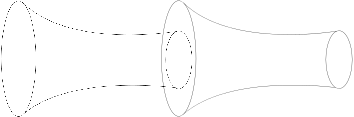
\includegraphics[scale=.2]{figures/method/funnel-composition}
  \centering
  \caption{Two funnels composed.}
\end{figure}

\section{TVLQR}

Tuning of the parameters in the \textit{TVLQR} algorithm.

\section{Simulations}

\subsection{Collision checking}

\subsection{Staying inside the funnels}

As a funnel is not simply the 2D-ellipse projected down into the plane. In fact
the funnel lives in 4D space, and as such the vehicle can leave the funnel, even
though it is inside the projected funnel in 2D space. Therefore the \rrtfunnel{}
algorithm checks at each step during the simulations that the vehicle stays
inside the verified funnels. This is done through inputting the vehicle's
current state into the quadratic Lyapunov function
\[
  {\bar{x}}^{T}S_{k}\bar{x} + \bar{x}s_{1} \bar{x} s_{2}
\]

\subsection{Expanding the size of the funnel by the size of the simulated vehicle}

The size of the vehicle in the model is in the original vehicle model in
\ref{TODO}, a single point, and as such, not accounted for in the funnel before
running simulations. Therefore the funnels have to be expanded in order for them
to accomodate the necessary robustness guarantees that are expected. However,
the size of the vehicle only affects the size of the funnel ellipsis projected
down into the xy-plane. Therefore first getting the projected size of the funnel
\[
  S_{p} = CSC^{T} (TODO - check)
\]
where
\[
  C =
  \begin{bmatrix}
    I & \mathbf{0} \\
    \mathbf{0} & \mathbf{0} \\
\end{bmatrix}
\]
and then expanding with the radii of the vehicle (TODO) using th
\[
                Sp = obj.funnels{i}.Sp{j};
                [VV,DD] = eig(Sp);
                l1 = 1/sqrt(DD(1,1)) + radius;
                l2 = 1/sqrt(DD(2,2)) + radius;
                % l3 = 1/sqrt(DD(3,3)) + radius;
                d1 = 1/l1^2;
                d2 = 1/l2^2;
                % d3 = 1/l3^2;
                D2 = diag([d1,d2]);
                Sp2 = VV*D2*VV';
                obj.funnels{i}.cS{j} = chol(Sp2);
\]

\section{Creating more motion primitives}

Although the base motion primitive library is pretty sparse, just like the
\rrtfunnel{} algorithm creates paths from stacking motion primitives, longer
motion primitives can be built \textit{for} the \rrtfunnel{} algorithm. This is
beneficial also, as it helps the algorithm expand quickly into the unsearched
parts of the searchspace, and therefore helps it regain some of the benefits of
the original \ac{RRT} algorithm.

(Downsides -- does not necessarily expand into other parts than the xy-plane).

\subsection{}

\section{Funnel-graph}

Even though the \rrtfunnel{} algorithm can work just fine with a collection of
funnels, and simply bruteforcing all funnels at the planning stage, it is
helpful to associate some kind of structure with the collection. In essence
associating the collection of funnels \(\mathcal{F}\) with some structure.
Giving the collection \(\mathcal{F}\) a tree structure, where each node in the
tree is reached, either through a funnel, a part of a funnel (which is also a
funnel), or a composition of funnels. Each funnel already has a set of nodes
associated with itself from the discretization taking place prior to funnel
creation as shown in figure \ref{fig:somefig}.

\begin{figure}
  \centering
  \begin{minipage}[b]{0.4\textwidth}
    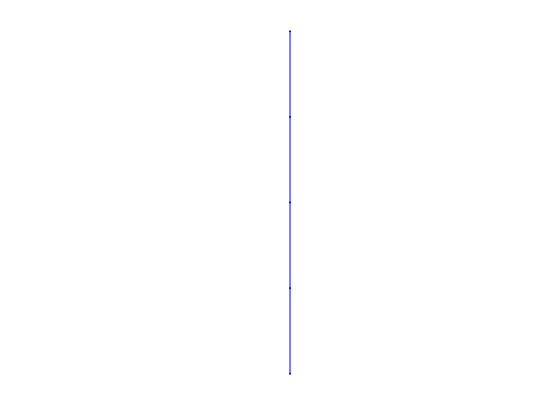
\includegraphics[width=\textwidth]{figures/method/trajectory-sampled}
    \caption{Trajectory sampled \# times (TODO)}
  \end{minipage}
  \hfill
  \begin{minipage}[b]{0.4\textwidth}
    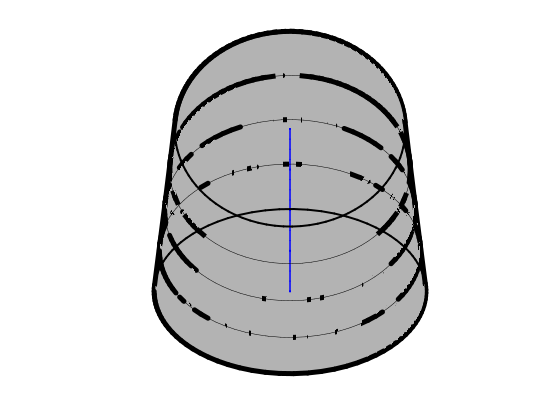
\includegraphics[width=\textwidth]{figures/method/funnel-sampled}
    \caption{The verified trajectory ellipsis overlaid at the sample times.}
  \end{minipage}
\end{figure}

For each funnel, in order to not only be able to compose funnels, but
sub-funnels, which means that at every point of every node in every funnel
composability with every other sample point in every other funnel has to be
checked. This is summed up more orderly in algorithm
\ref{alg:create-funnel-graph}, where a funnel is a vertice in the graph, and an
ordered pair of funnels \(\left( F_{i}, F_{j} \right)\) is an edge. Composition
of funnels is checked in the same way as in \ref{def:funnel-composition}.

\begin{algorithm}
  \caption{Create Funnel Graph}
  \label{alg:create-funnel-graph}
  \DontPrintSemicolon \SetAlgoNoLine

  \KwIn{\(\mathcal{F}\) -- The basis set of funnels computed around the nominal
    trajectories.} \KwOut{\(\mathcal{G}(\mathcal{F})\) -- Directed graph
    representing the composability of funnels.}

  \ForEach{\(F_{i} \in \mathcal{F}\)} { \ForEach{\(F_{j} \in \mathcal{F}\)} {
      \ForEach{\(t_{k} \in F_{i}\)} { \ForEach{\(t_{l} \in F_{j}\)} {
          \If{\(F_{i}(t_{k}) \subset F_{j}(t_{l})\)} { \(\mathcal{G}
            \leftarrow{} \left( F_{i}(t_{k}), F_{j}(t_{l}) \right)\) } \; } \; }
      \; }\; }\;

\end{algorithm}

\section{RRT-section}

